\subsubsection{从微分的角度看隐函数定理}

\subparagraph*{Method 2}

$F(x_0,\cdot)=0\leadsto y_0$ aim: $F(x,\cdot)=0$

$\begin{matrix}
        y_{n+1}=y_n-\frac{F(x,y_n)}{\frac{\partial F}{\partial y}(x,y_n)} \\
        \downarrow                                                        \\
        y_{n+1}=y_n-\left.(J_yF)^{-1}\right|_{(x,y_n)}F(x,y_n)
    \end{matrix}$\quad\raisebox{-0.5\height}{
\includegraphics[height=3cm]{chapters/09/03/0106}}


Step 1. $y_0$ is an approximate solution to $F(x,\cdot)=0$ for $x$ sufficiently close to $x_0$,
$$y_{n+1}\triangleq y_n-\frac{F(x,y_n)}{\frac{\partial F}{\partial y}(x_0,y_0)}$$

$(y_{n+1}-y_n)=(y_n-y_{n-1})-\frac{F(x,y_n)-F(x,y_{n-1})}{\frac{\partial F}{\partial y}(x_0,y_0)}=(y_n-y_{n-1})-\frac{\frac{\partial F}{\partial y}(x,\tilde{y_n})}{\frac{\partial F}{\partial y}(x_0,y_0)}(y_n-y_{n-1})$

$\rightarrow|y_{n+1}-y_n|\leq\frac{1}{2}|y_n-y_{n-1}|$\\
$y\mapsto y-(J_yF)^{-1}F(x,y)$\\
$y_1=y_0-F(x,y_0)$\\
$|y_1-y_0|=|F(x,y_0)|<\frac{1}{4}$\\
$\sqrt{(x-x_0)^2+(y_1-y_0)^2}<\frac{1}{4}$

\begin{thm}[Implicit Function Theorem]
    Let $D\subseteq\mathbb{R}^n\times\mathbb{R}^m$ be an open set, $M_0=(x_0,y_0)\in D$. If the vector-valued function $F:\,D\to\mathbb{R}^m$ satisfies\begin{enumerate}
        \item $F\in C^1(D)$
        \item $F(x_0,y_0)=0$
        \item $\left.(J_yF)\right|_{(x_0,y_0)}$ invertible
    \end{enumerate}
    $\implies$\begin{enumerate}
        \item $\exists$ neighborhood $I$ of $x_0$ in $\mathbb{R}^n$, neighborhood $J$ of $y_0$ in $\mathbb{R}^m$, s.t. $F(x,y)=0$ determines an implicit function $y:\,I\to J$
        \item $y=y(x)$ is $C^1$
        \item $dy|_x=-(d_yF)^{-1}|_{(x,y(x))}\circ(d_xF)|_{(x,y(x))}$
    \end{enumerate}
\end{thm}

Explanation: $dF|_{(x,y)}$: $\mathbb{R}^n\times\mathbb{R}^m\to\mathbb{R}^m$ is a linear map

$\leadsto$ Restriction: \allbold{partial differential} $\begin{cases}
        d_xF|_{(x,y)}=\left.dF|_{(x,y)}\right|_{\mathbb{R}^n\times\{0\}}\text{: }\mathbb{R}^n\to\mathbb{R}^m\text{\allbold{ linear}} \\
        d_yF|_{(x,y)}=\left.dF|_{(x,y)}\right|_{\{0\}\times\mathbb{R}^m}\text{: }\mathbb{R}^m\to\mathbb{R}^m\text{\allbold{ linear}}
    \end{cases}$

In terms of Jacobi matrix,
$$
    d_yF\sim\underset{J_yF}{\begin{pmatrix}
            \frac{\partial F_1}{\partial y_1} & \cdots & \frac{\partial F_1}{\partial y_m} \\
            \vdots                            &        &                                   \\
            \frac{\partial F_m}{\partial y_1} & \cdots & \frac{\partial F_m}{\partial y_m}
        \end{pmatrix}},\,d_xF\sim\underset{J_xF}{\begin{pmatrix}
            \frac{\partial F_1}{\partial x_1} & \cdots & \frac{\partial F_1}{\partial x_n} \\
            \vdots                            &        &                                   \\
            \frac{\partial F_m}{\partial x_1} & \cdots & \frac{\partial F_m}{\partial x_n}
        \end{pmatrix}}\substack{\implies}\begin{pmatrix}
        \frac{\partial y_1}{\partial x_1} & \cdots & \frac{\partial y_1}{\partial x_n} \\
        \vdots                            &        &                                   \\
        \frac{\partial y_m}{\partial x_1} & \cdots & \frac{\partial y_m}{\partial x_n}
    \end{pmatrix}=-(J_yF)^{-1}\cdot (J_xF)
$$

\begin{center}
    
\includegraphics[width=\columnwidth]{chapters/09/03/0107.jpg}
\end{center}

\begin{pf}
    Given $x\in\mathbb{R}^n$. Construct a map $G^*:\,\mathbb{R}^m\to\mathbb{R}^m$, $y\mapsto (y-(J_yF)|_{(x_0,y_0)})^{-1}F(x,y)$

    1. $G^*(y')-G^*(y'')=y'-y''-J^{-1}(F(x,y')-F(x,y''))$

    $G^*(y)=y\iff F(x,y)=0$

    $F'(x,y_1',\dots,y_m')-F'(x,y_1'',\dots,y_m'')=\frac{\partial F'}{\partial y'}(y_1'-y_1'')+\dots+\frac{\partial F'}{\partial y_m'}(y_m'-y_m'')$

    $J^{-1}(F(x,y')-F(x,y''))\rightarrow\begin{pmatrix}
            \frac{\partial F^1}{\partial y_1} & \cdots & \frac{\partial F^1}{\partial y_m} \\
            \vdots                            &        &                                   \\
            \frac{\partial F^m}{\partial y_1} & \cdots & \frac{\partial F^m}{\partial y_m}
        \end{pmatrix}\begin{pmatrix}
            y_1'-y_1'' \\
            \vdots     \\
            y_m'-y_m''
        \end{pmatrix}$

    $\implies|G^*(y')-G^*(y'')|\leq\frac{1}{2}|y'-y''|$

    2. $G^*(\overline{B(y_0,\delta)})\subseteq\overline{B(y_0,\delta)}$
\end{pf}

% 20260407

\paragraph*{Several low dimensional cases}

\begin{enumerate}
    \item $F:\,\mathbb{R}^3\to\mathbb{R}$ is $C^1$

          $\begin{cases}
                  F(x_0,y_0,z_0)=0 \\
                  \left.\frac{\partial F}{\partial z}\right|_{(x_0,y_0,z_0)}\neq 0
              \end{cases}\overset{\text{Implicit Function Thm}}{\leadsto}$\quad\raisebox{-0.5\height}{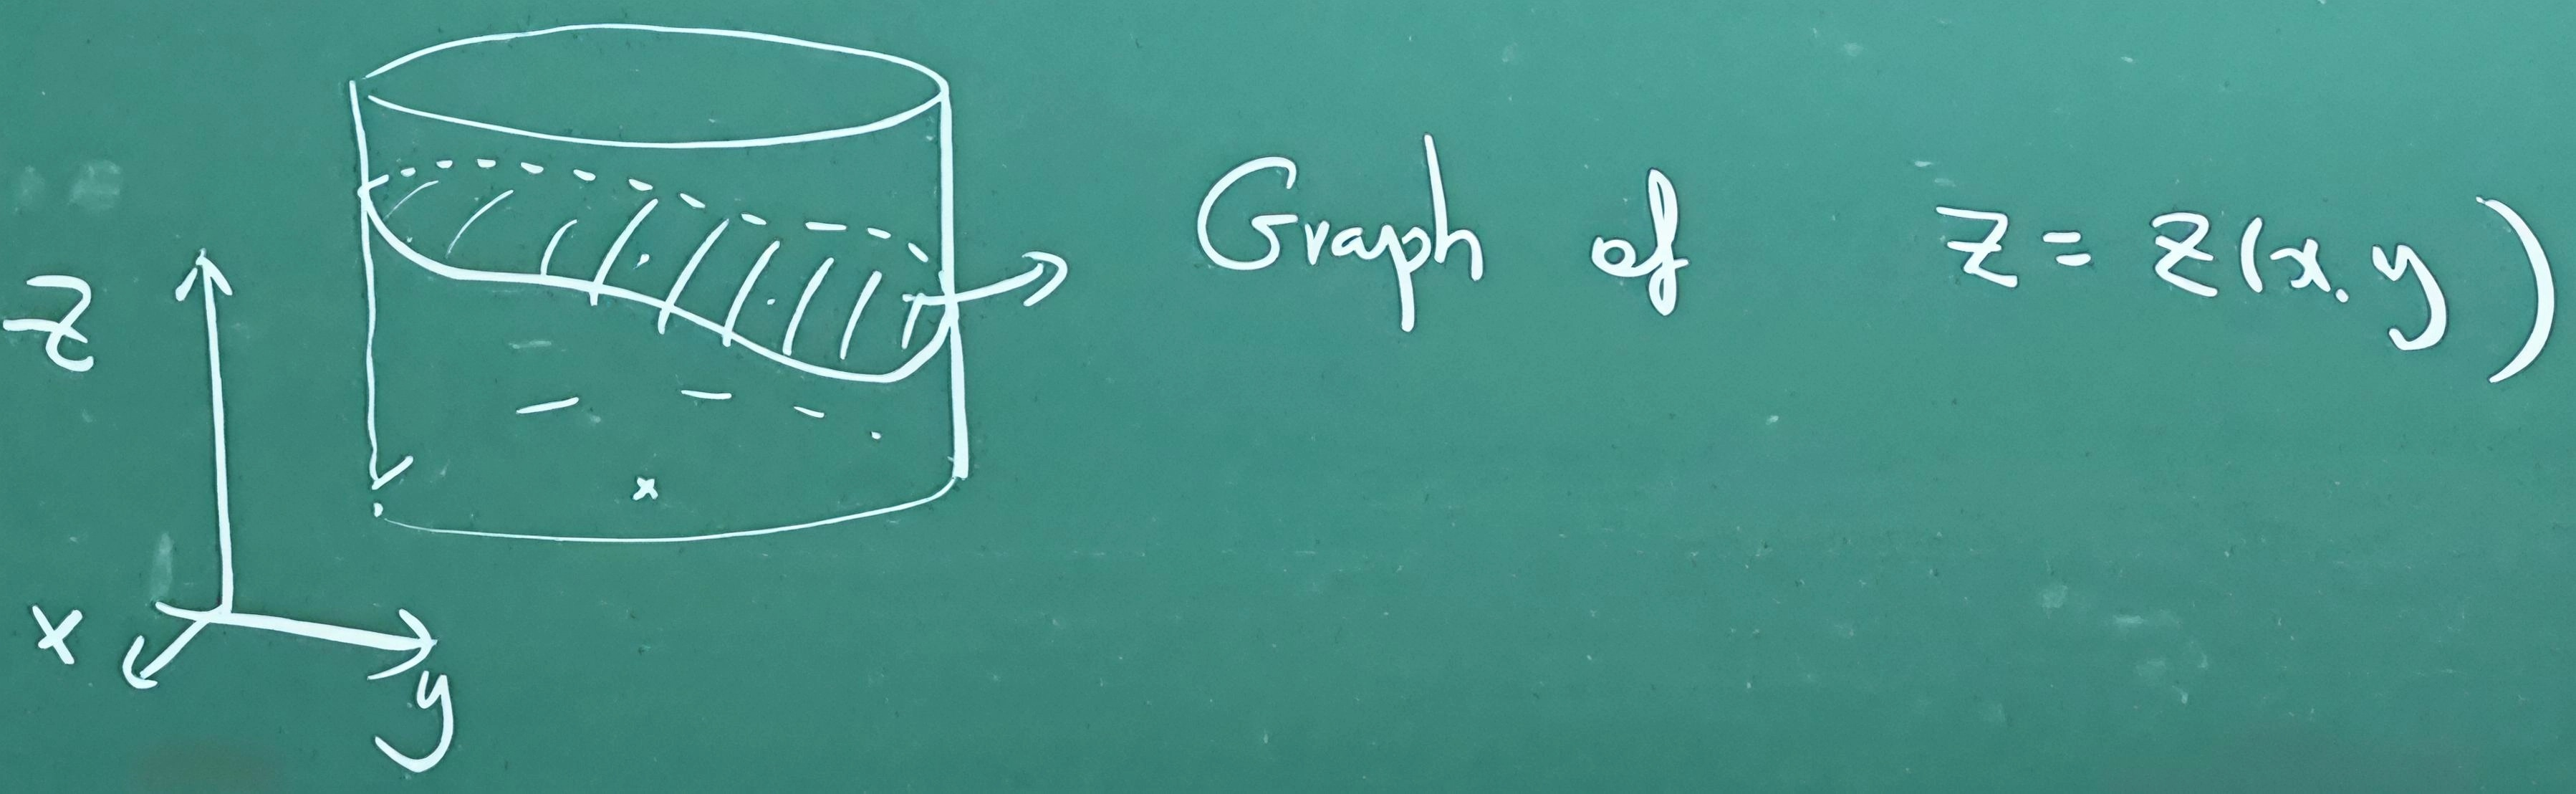
\includegraphics[height=2cm]{chapters/09/03/0108}}

          \begin{itemize}
              \item $\exists$ local implicit function $z=z(x,y)$ is $C^1$
              \item Differentiable $F(x,y,z(x,y))=0$ directly $\frac{\partial F}{\partial x}dx+\frac{\partial F}{\partial y}dy+\frac{\partial F}{\partial z}dz=0\implies dz=-\frac{1}{\frac{\partial F}{\partial z}}\left(\frac{\partial F}{\partial x}dx+\frac{\partial F}{\partial y}dy\right)$
          \end{itemize}

          \begin{rmk}
              Implicit Function Thm provides a natural parameterization (locally, $C^1$) for the surface $\{(x,y,z)\in\mathbb{R}^3\mid F(x,y,z)=0\}$:

              $$(x,y)\mapsto(x,y,z(x,y))$$

              \begin{example}
                  $x^2+y^2+z^2=1$

                  $\leadsto$ Around $z\neq0$, $(x,y)\to(x,y,z(x,y))=\begin{cases}
                          (x,y,\sqrt{1-x^2-y^2}) \\
                          (x,y,-\sqrt{1-x^2-y^2})
                      \end{cases}$\quad\raisebox{-0.5\height}{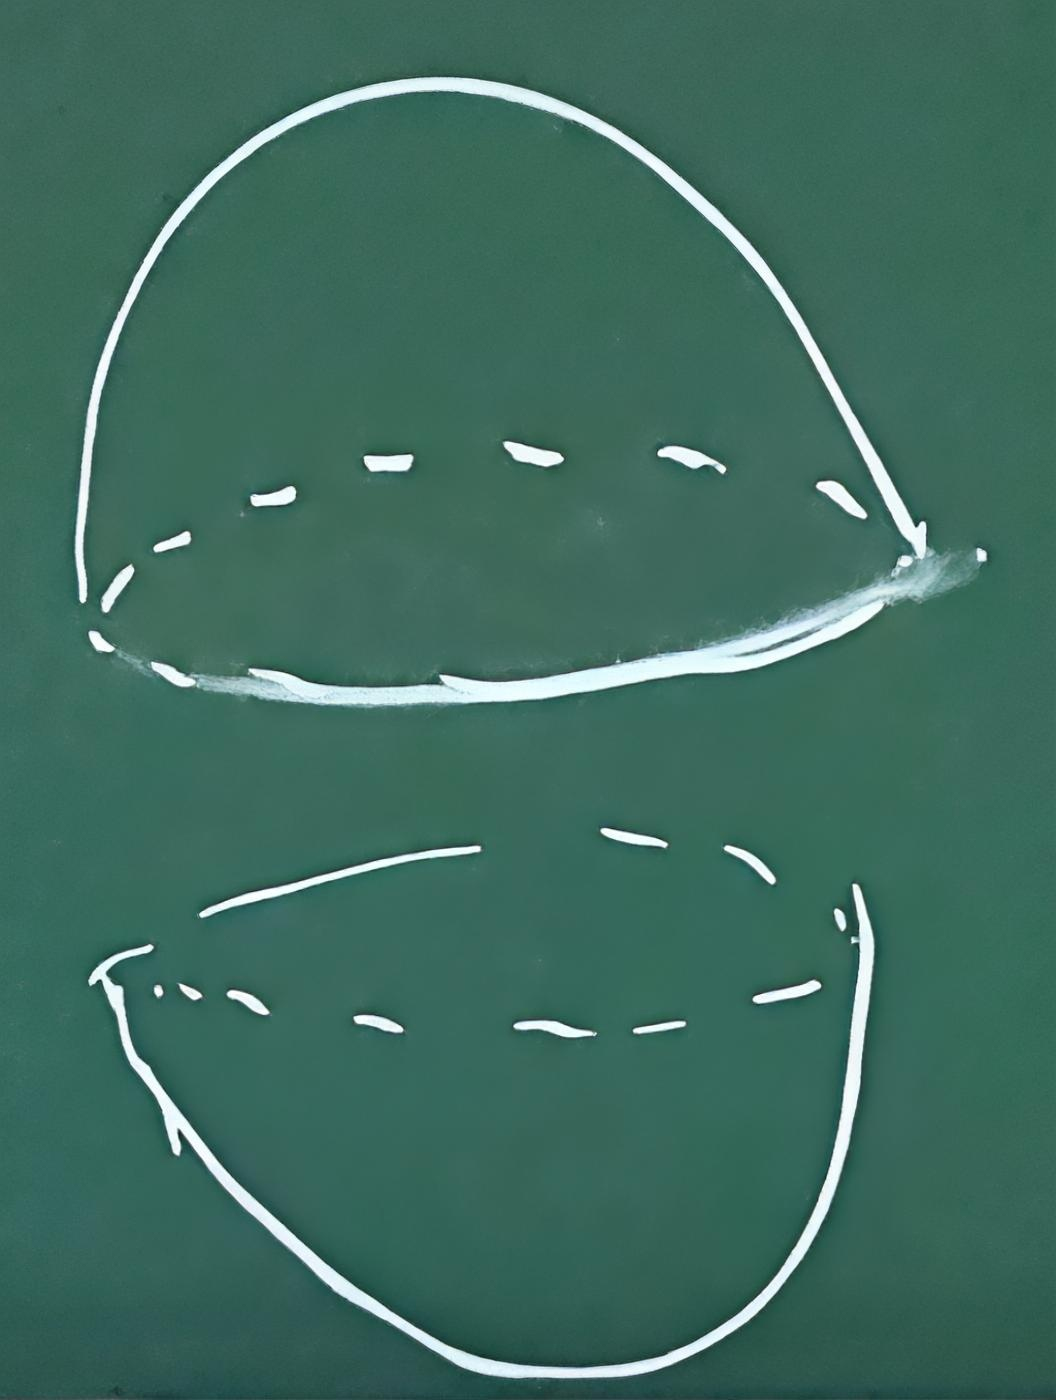
\includegraphics[height=2cm]{chapters/09/03/0109}}

              \end{example}
          \end{rmk}

          If $\nabla F|_{(x_0,y_0,z_0)}\neq0$, then $\underset{\substack{\downarrow\\x=x(y,z)\\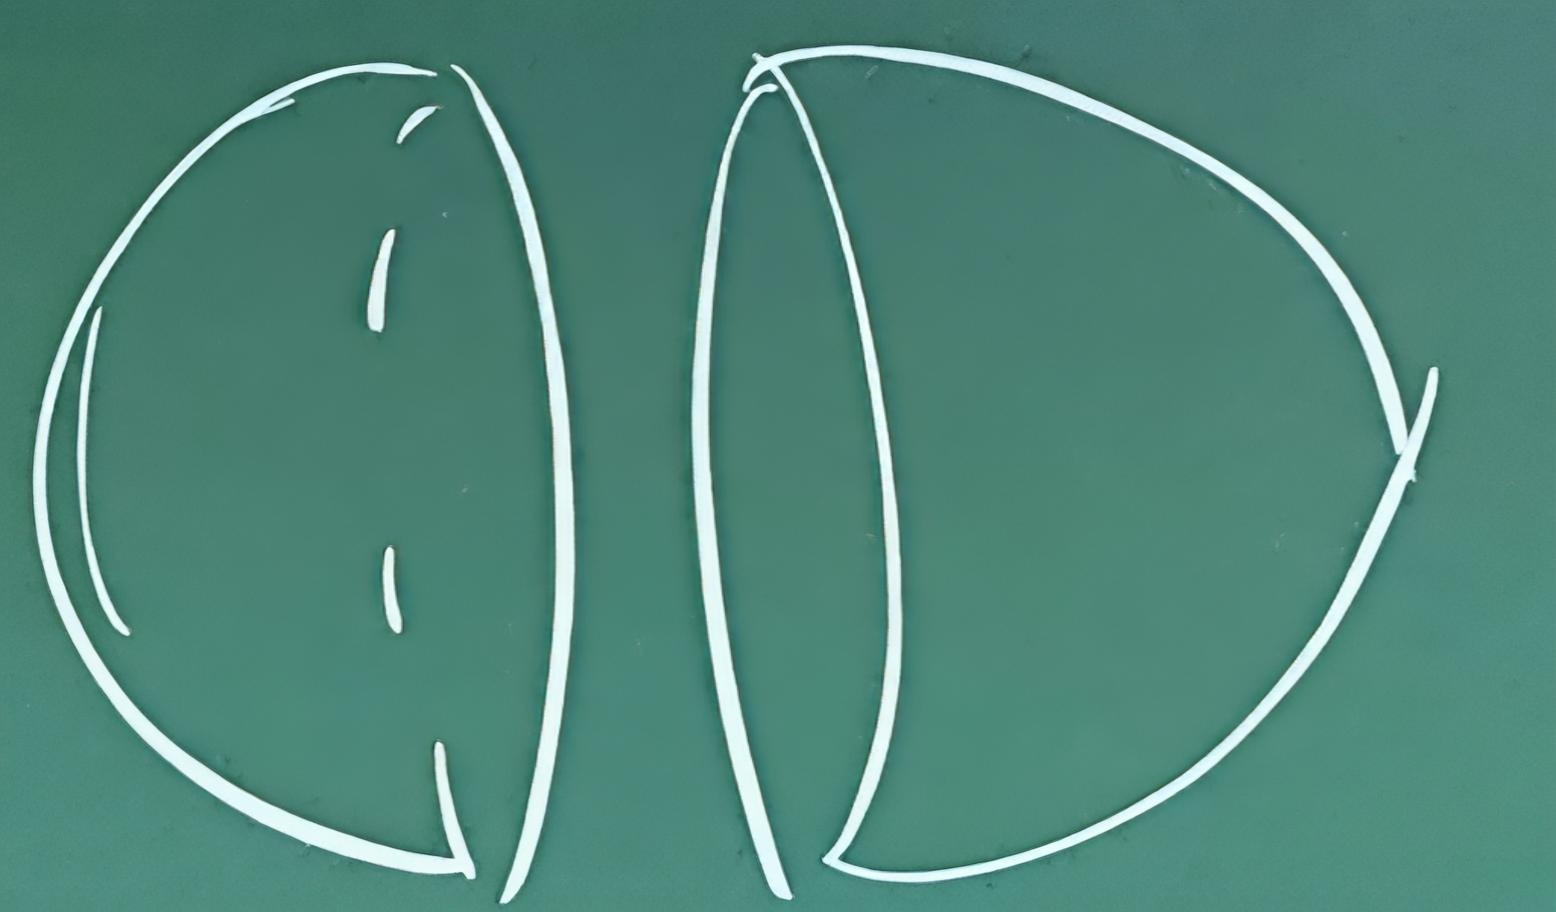
\includegraphics[height=1cm]{chapters/09/03/0110}}}{\left.\frac{\partial F}{\partial x}\right|_{(x_0,y_0,z_0)}\neq0}$, or $\underset{\substack{\downarrow\\y=y(x,z)\\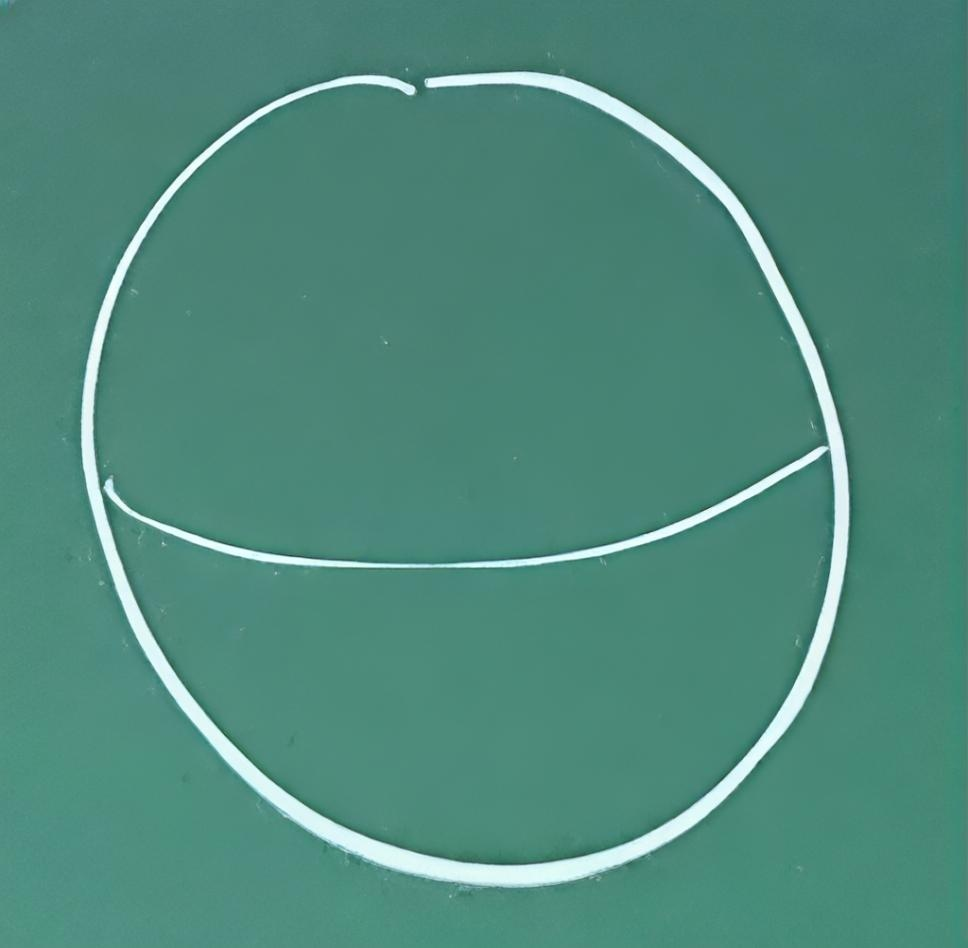
\includegraphics[height=1cm]{chapters/09/03/0111}}}{\left.\frac{\partial F}{\partial y}\right|_{(x_0,y_0,z_0)}\neq0}$, or $\underset{\substack{\downarrow\\z=z(x,y)\\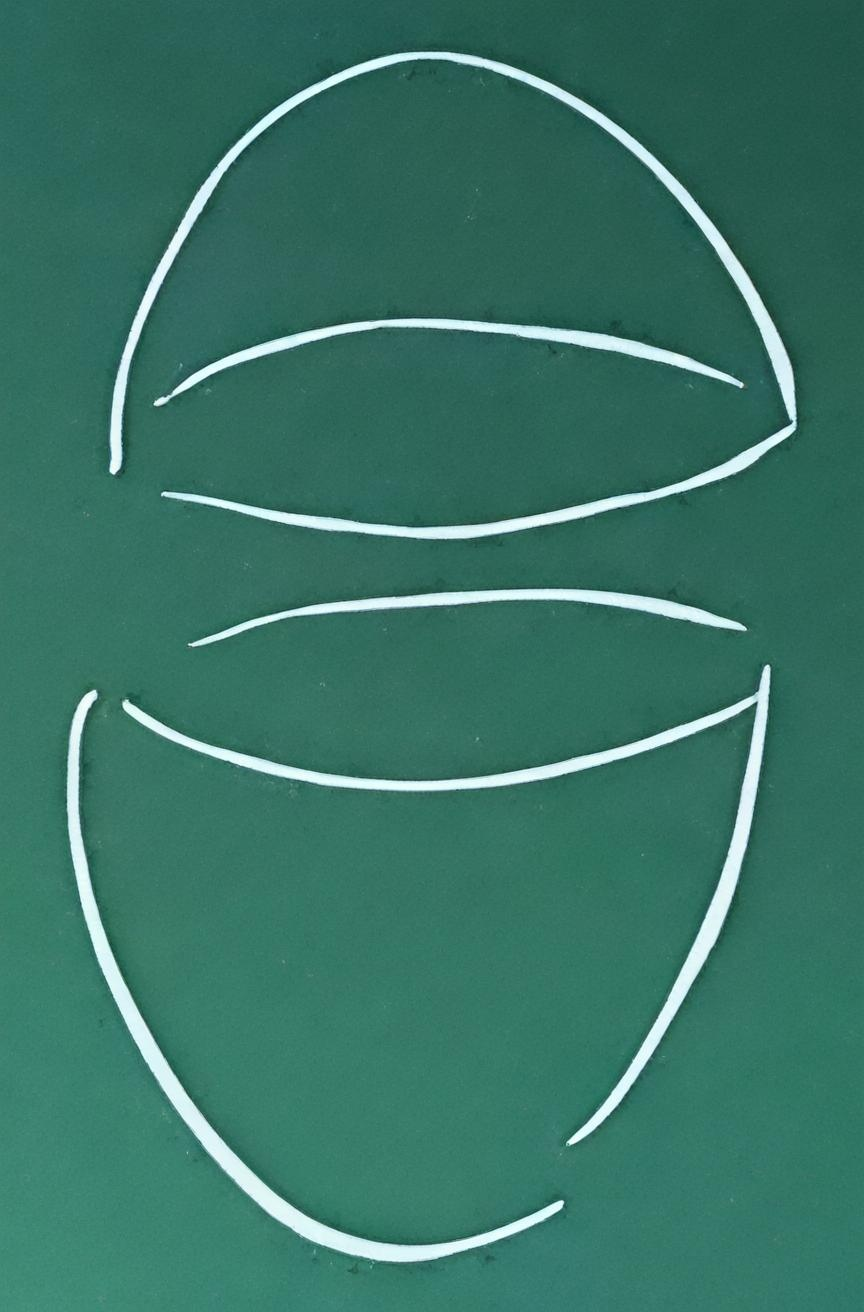
\includegraphics[height=1cm]{chapters/09/03/0112}}}{\left.\frac{\partial F}{\partial z}\right|_{(x_0,y_0,z_0)}\neq0}$

          manifold

          \raisebox{-0.5\height}{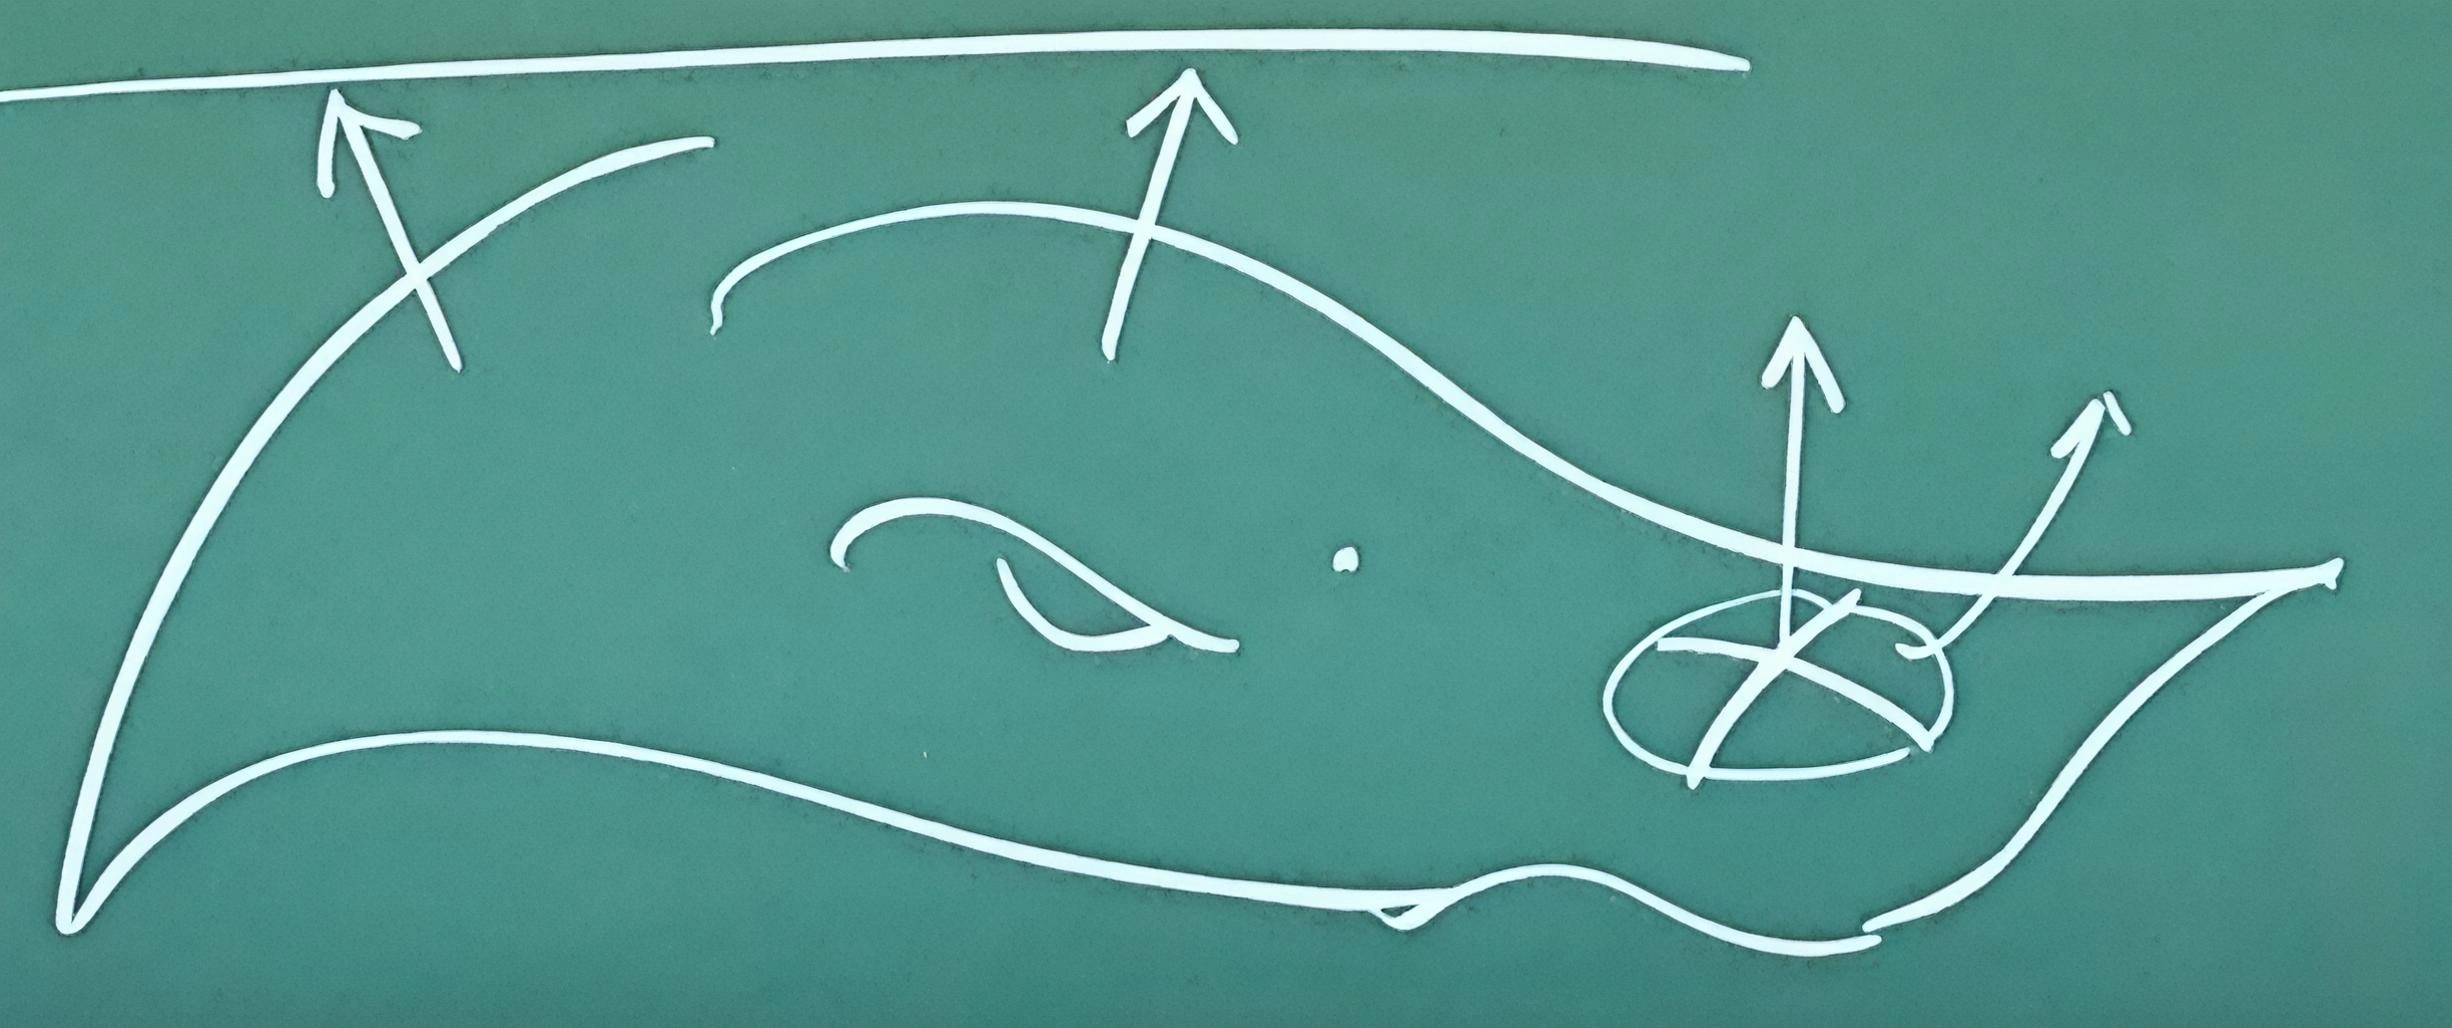
\includegraphics[height=2cm]{chapters/09/03/0113}}\quad$\substack{(x,y,z(x,y))\\F=0}\rightarrow\substack{r_x=(1,0,\frac{\partial z}{\partial x})\\r_y=(0,1,\frac{\partial z}{\partial y})}\implies r_x,r_y\bot \nabla F$

          \begin{rmk}
              If $\nabla F|_{(x_0,y_0,z_0)}\neq0$, $F|_{(x_0,y_0,z_0)}$, we cannot use Implicit Function Thm.

              \begin{example}
                  \raisebox{-0.5\height}{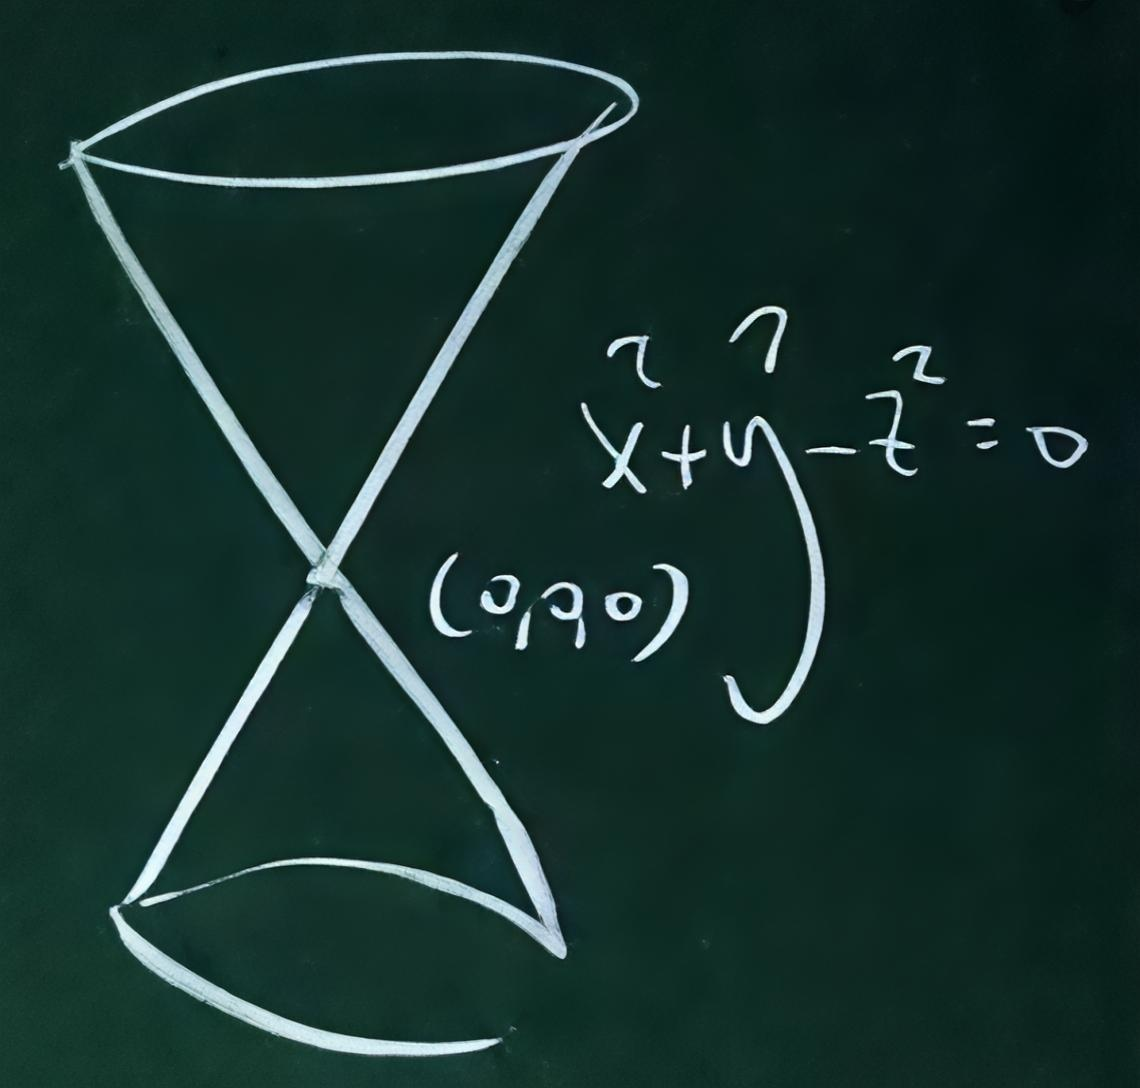
\includegraphics[height=2cm]{chapters/09/03/0114}}
              \end{example}
          \end{rmk}
    \item $F,G:\,\mathbb{R}^3\to\mathbb{R}$, $C^1$, consider $\{(x,y,z)\in\mathbb{R}^3\mid F(x,y,z)=0,G(x,y,z)=0\}$

          Consider $\substack{\mathbb{R}^4\to\mathbb{R}^2\\(x,y,z)\mapsto(F(x,y,z),G(x,y,z))}$.

          $\rightarrow$ Jacobi matrix $JF=\begin{pmatrix}
                  \frac{\partial F}{\partial x} & \frac{\partial F}{\partial y} & \frac{\partial F}{\partial z} \\
                  \frac{\partial G}{\partial x} & \frac{\partial G}{\partial y} & \frac{\partial G}{\partial z}
              \end{pmatrix}$.

          If $\operatorname{rank}(JF|_{(x_0,y_0,z_0)})=2$, then $\underset{\substack{\downarrow\\(y,z)=(y(x),z(x))}}{\frac{\partial(F,G)}{\partial(y,z)}}\neq 0$, or $\underset{\substack{\downarrow\\(z,x)=(z(y),x(y))}}{\frac{\partial(F,G)}{\partial(z,x)}}\neq 0$, or $\underset{\substack{\downarrow\\(x,y)=(x(z),y(z))}}{\frac{\partial(F,G)}{\partial(x,y)}}\neq 0$

          \begin{center}
              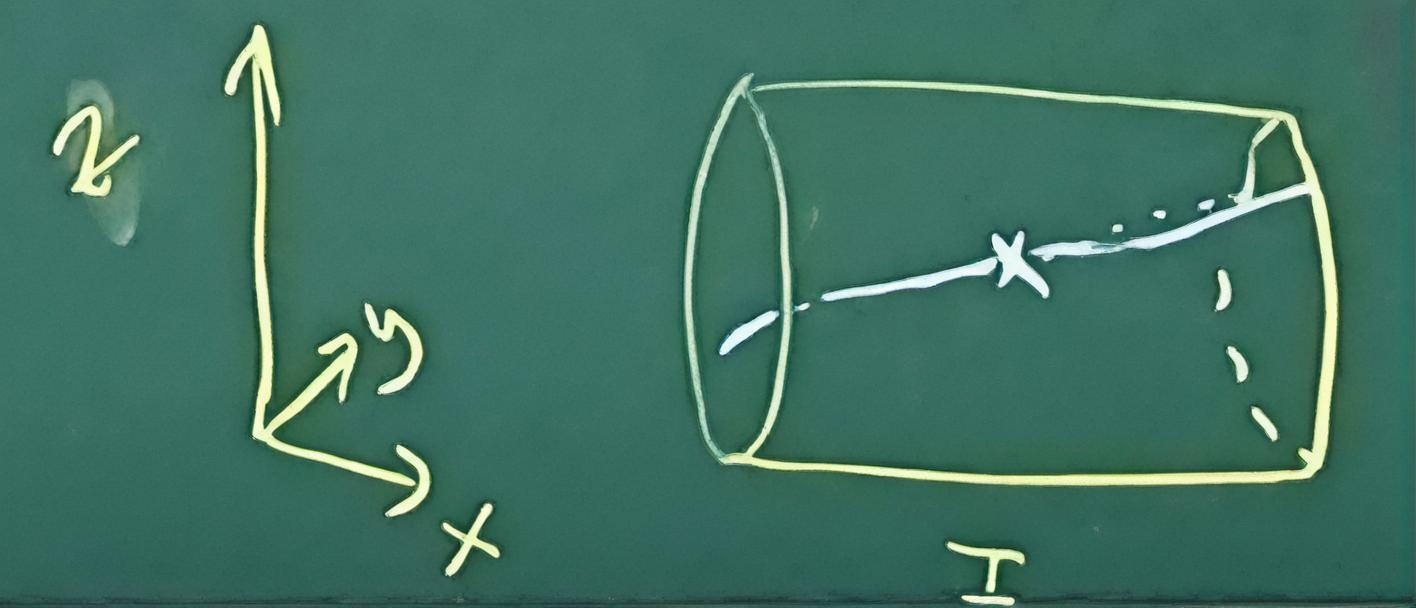
\includegraphics[height=2cm]{chapters/09/03/0115}
          \end{center}

          Diff. $\begin{cases}
                  F(x,y(x),z(x))=0 \\
                  G(x,y(x),z(x))=0
              \end{cases}$

          \begin{align*}
              (JF)\begin{pmatrix}
                      dx \\dy\\dz
                  \end{pmatrix}=0
               & \implies\begin{pmatrix}
                             \frac{\partial F}{\partial x} \\\frac{\partial G}{\partial x}
                         \end{pmatrix}dx
              +\begin{pmatrix}
                   \frac{\partial F}{\partial y} & \frac{\partial F}{\partial z} \\
                   \frac{\partial G}{\partial y} & \frac{\partial G}{\partial z}
               \end{pmatrix}
              \begin{pmatrix}
                  dy \\dz
              \end{pmatrix}=0                                                         \\
               & \implies\begin{pmatrix}
                             dy \\dz
                         \end{pmatrix}
              =-\begin{pmatrix}
                    \frac{\partial F}{\partial y} & \frac{\partial F}{\partial z} \\
                    \frac{\partial G}{\partial y} & \frac{\partial G}{\partial z}
                \end{pmatrix}^{-1}
              \begin{pmatrix}
                  \frac{\partial F}{\partial x} \\\frac{\partial G}{\partial x}
              \end{pmatrix}dx
          \end{align*}

          $\rightarrow$ Local parameterization for the curve $\{F=0\}\cap\{G=0\}$

          $x\mapsto(x,y(x),z(x))$\quad$\begin{pmatrix}
                  a & b \\
                  c & d
              \end{pmatrix}^{-1}
              =\frac{1}{ad-bc}\begin{pmatrix}
                  d  & -b \\
                  -c & a
              \end{pmatrix}$

          \begin{align*}
              \begin{pmatrix}
                  \frac{dy}{dx} \\\frac{dz}{dx}
              \end{pmatrix}
               & =-\frac{1}{\frac{\partial(F,G)}{\partial(y,z)}}\begin{pmatrix}
                                                                    \frac{\partial G}{\partial z}  & -\frac{\partial F}{\partial z} \\
                                                                    -\frac{\partial G}{\partial y} & \frac{\partial F}{\partial y}
                                                                \end{pmatrix}
              \begin{pmatrix}
                  \frac{\partial F}{\partial x} \\\frac{\partial G}{\partial x}
              \end{pmatrix}                                                                 \\
               & =-\frac{1}{\frac{\partial(F,G)}{\partial(y,z)}}\begin{pmatrix}
                                                                    -\frac{\partial(F,G)}{\partial(z,x)} \\-\frac{\partial(F,G)}{\partial(x,y)}
                                                                \end{pmatrix}
          \end{align*}

          $\rightarrow r_x=(1,\frac{dy}{dx},\frac{dz}{dx})=\frac{1}{\frac{\partial(F,G)}{\partial(y,z)}}(\frac{\partial(F,G)}{\partial(y,z)},\frac{\partial(F,G)}{\partial(z,x)},\frac{\partial(F,G)}{\partial(x,y)})=\frac{1}{\frac{\partial(F,G)}{\partial(y,z)}}(\nabla F\times\nabla G)$\quad\raisebox{-0.5\height}{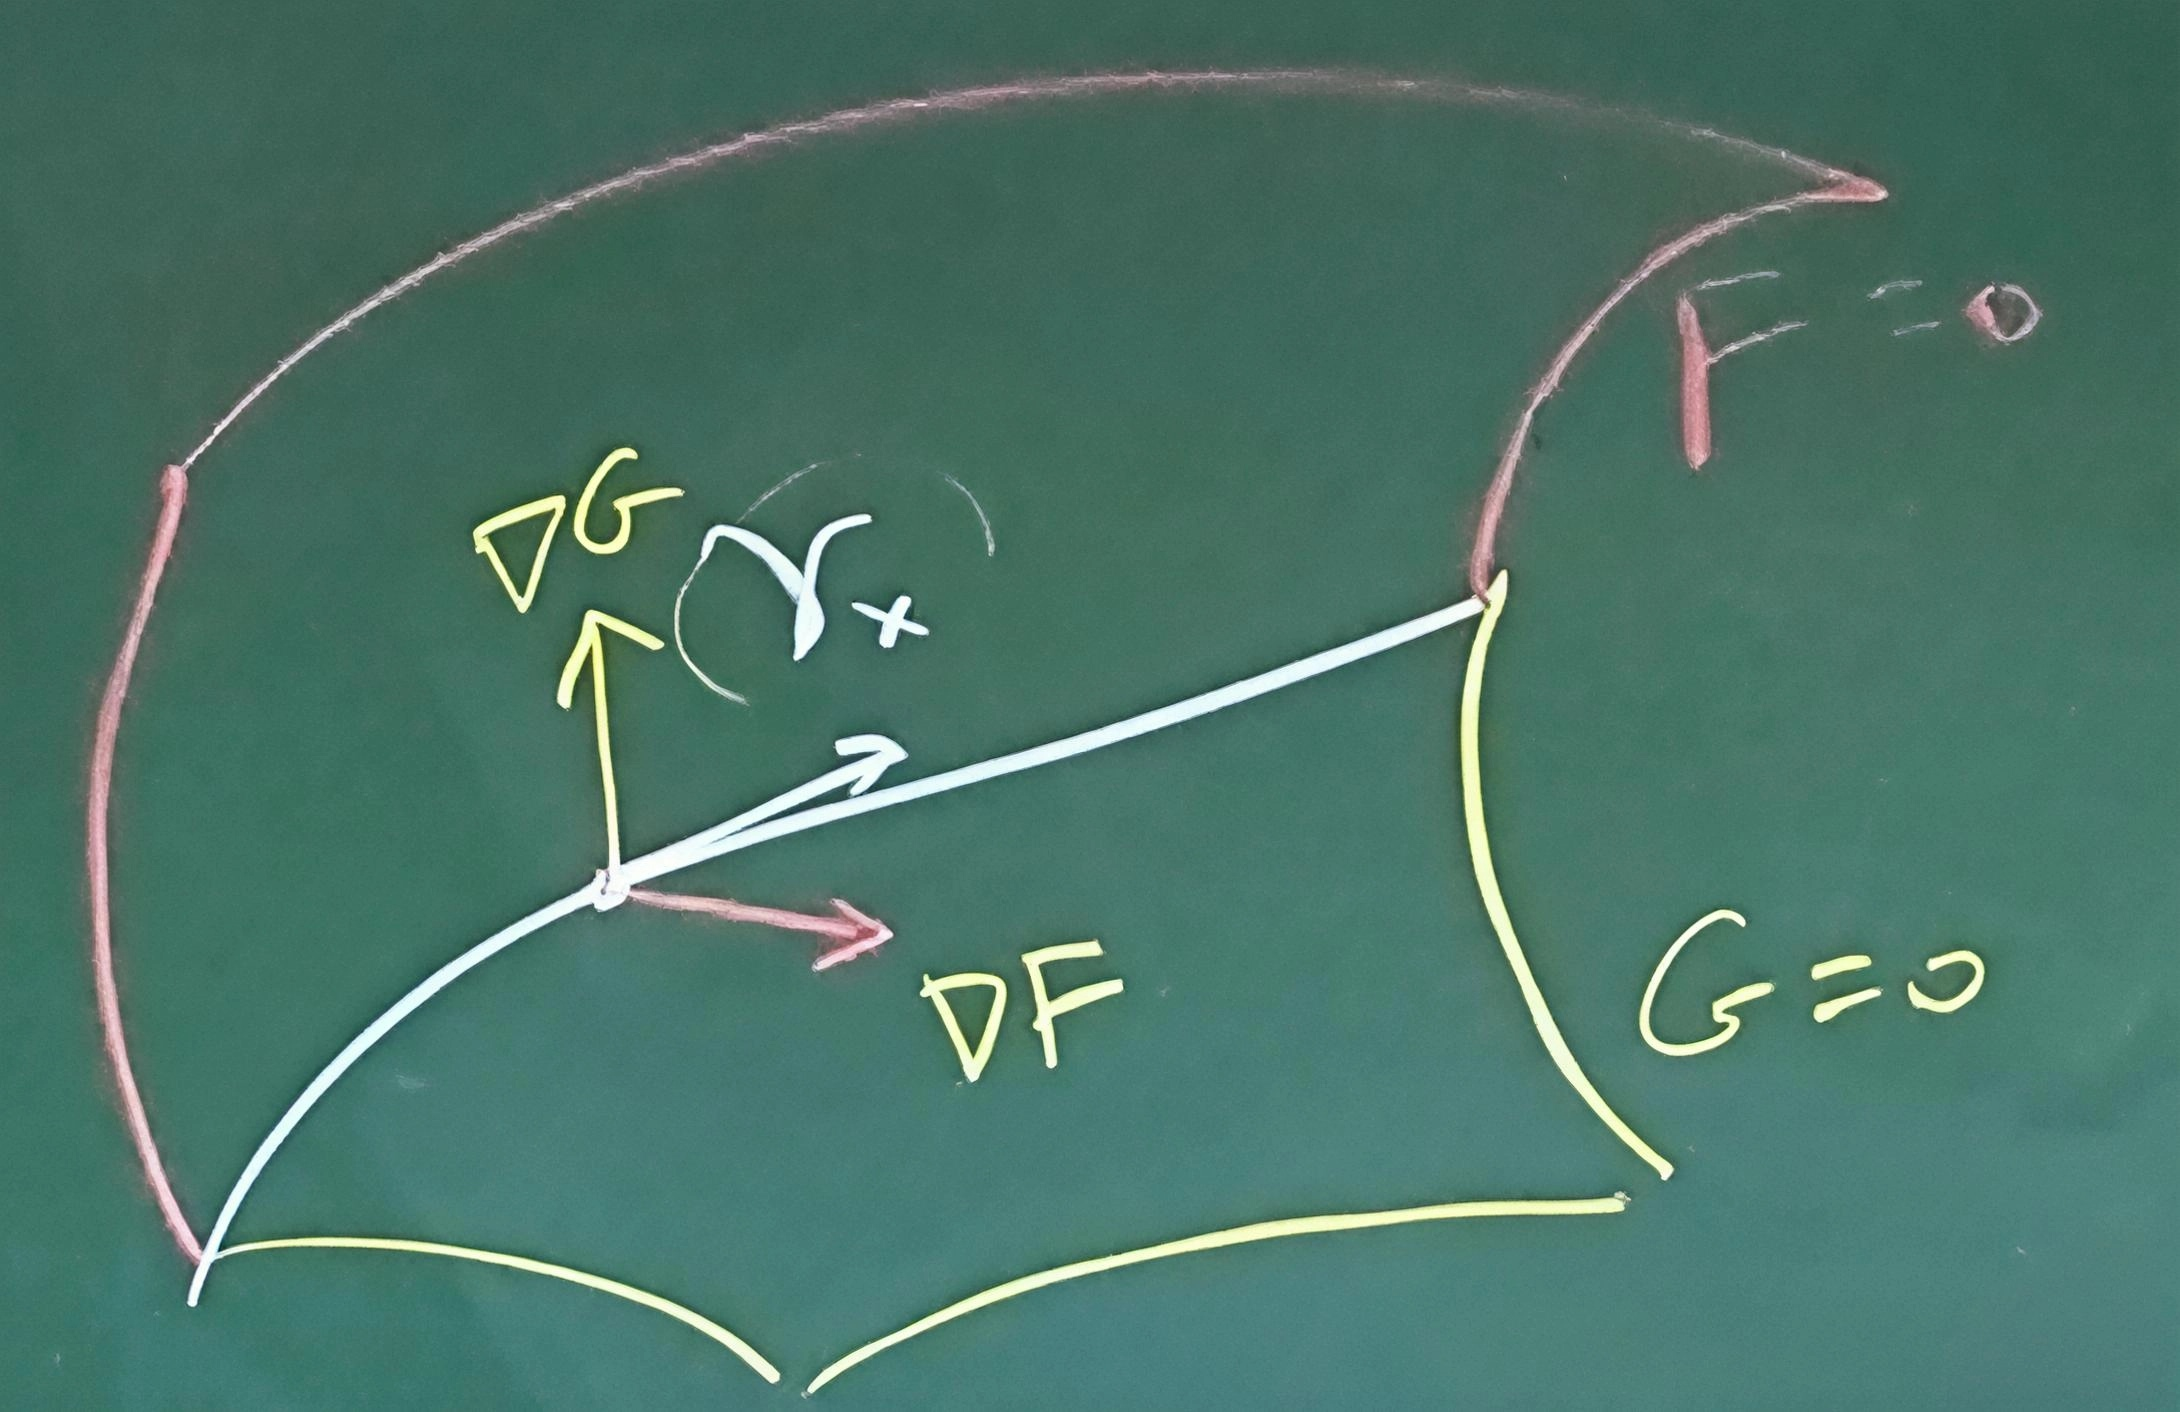
\includegraphics[height=2cm]{chapters/09/03/0116}}

          \begin{example}
              The equations $\substack{u^2-v+x=0\quad u+v^2-y=0\\(x,y)\mapsto(u(x,y),v(x,y))}$ determines an implicit function.

              Find $\frac{\partial u}{\partial x},\frac{\partial u}{\partial y}$

              Sol. Differentiate the two equations,
              \begin{align*}
                  \begin{cases}
                      2udu-dv+dx=0 \\
                      du+2vdv-dy=0
                  \end{cases}
                   & \implies\begin{pmatrix}
                                 2u & -1 \\
                                 1  & 2v
                             \end{pmatrix}\begin{pmatrix}du\\dv\end{pmatrix}=\begin{pmatrix}-dx\\dy\end{pmatrix} \\
                   & \implies\begin{pmatrix}du\\dv\end{pmatrix}
                  =\frac{1}{1+4uv}\begin{pmatrix}
                                      2v & 1  \\
                                      -1 & 2u
                                  \end{pmatrix}\begin{pmatrix}-dx\\dy\end{pmatrix}                               \\
                   & \quad=\frac{1}{1+4uv}\begin{pmatrix}
                                              -2vdx+dy \\
                                              dx+2udy
                                          \end{pmatrix}
              \end{align*}

              Therefore, $\frac{\partial u}{\partial x}=-\frac{2v}{1+4uv}$, $\frac{\partial u}{\partial y}=\frac{1}{1+4uv}$
          \end{example}
\end{enumerate}